\section{Preliminary} \label{sec:related}




\subsection{Test-Time Training}

Consider a one-dimensional sequence of $N$ tokens
$\mathbf{x} = [x_1, x_2, \dots, x_N]$, where each token $x_i \in \mathbb{R}^d$. 
Following attention formulation, 
each input tokens $x_i$ is projected into query ($q_i$), key ($k_i$), and value ($v_i$) vectors. 
For clarity, we assume all these vectors $q_i, k_i, v_i \in \mathbb{R}^d$.

Test-Time Training (TTT)~\cite{sun2024learning} introduces a neural network with rapidly adaptable weights---called \textit{fast weights}~\cite{schlag2021linear}---that are updated during 
both training and inference to dynamically store context information. 
This contrasts with the \textit{slow weights} (i.e., model parameters) that are frozen during inference.
Formally, TTT defines fast weights in the form of a neural network:
$f_W(\cdot): \mathbb{R}^d \rightarrow \mathbb{R}^d$ parameterized by the fast weights $W$,  and it involves two primary operations:
\begin{equation}
\textbf{Update operation:} \quad W \leftarrow W - \eta \nabla_{W} \mathcal{L}\big(f_W(k), v\big)
\label{eq:ttt_update}
\end{equation}
where $\mathcal{L}(\cdot,\cdot)$ is a loss function between the transformed key  $f_W(k)$ and the value $v$, commonly Mean Squared Error, designed to encourage the network to associate keys with corresponding values. 
$\eta$ is the learning rate.
Intuitively, this learning objective is to encode the KV cache into a neural memory with fixed state size as \emph{accurate} as possible~\cite{wang2025testtimeregressionunifyingframework}.
\begin{equation}
\textbf{Apply operation:}\quad \quad \quad
o = f_W(q),\quad 
\label{eq:ttt_apply}
\end{equation}
where the updated fast weights $W$ are used to compute the output vector $o$ given the query $q$.
The per-token TTT layer iteratively perform the update and apply operations on each token $x_i$ in sequence.




\subsection{Challenges in Efficient Implementation}
\label{sec:efficiency_challenge}

Frequent online update of fast weights is inefficient due to memory bandwidth limitations. Consequently, previous works~\cite{sun2023retentive, gu2023mamba, yang2024gated, qinvarious, yangparallelizing} often employ customized kernels that keep fast weights in SRAM across updates to reduce memory load. 
However, this strategy typically requires fast weights to evolve mostly independently within SMs to reduce communications, which is not valid for large nonlinear states (e.g., the nonlinear SwiGLU fast weight in Sect.~\ref{sec:ttt_layer} and the Muon update in Sec.~\ref{sec:update_rule}).   Moreover, developing such kernel code is cumbersome, with far longer development cycles than native PyTorch code, hindering rapid research exploration.



\begin{figure}[t!]
    \centering
    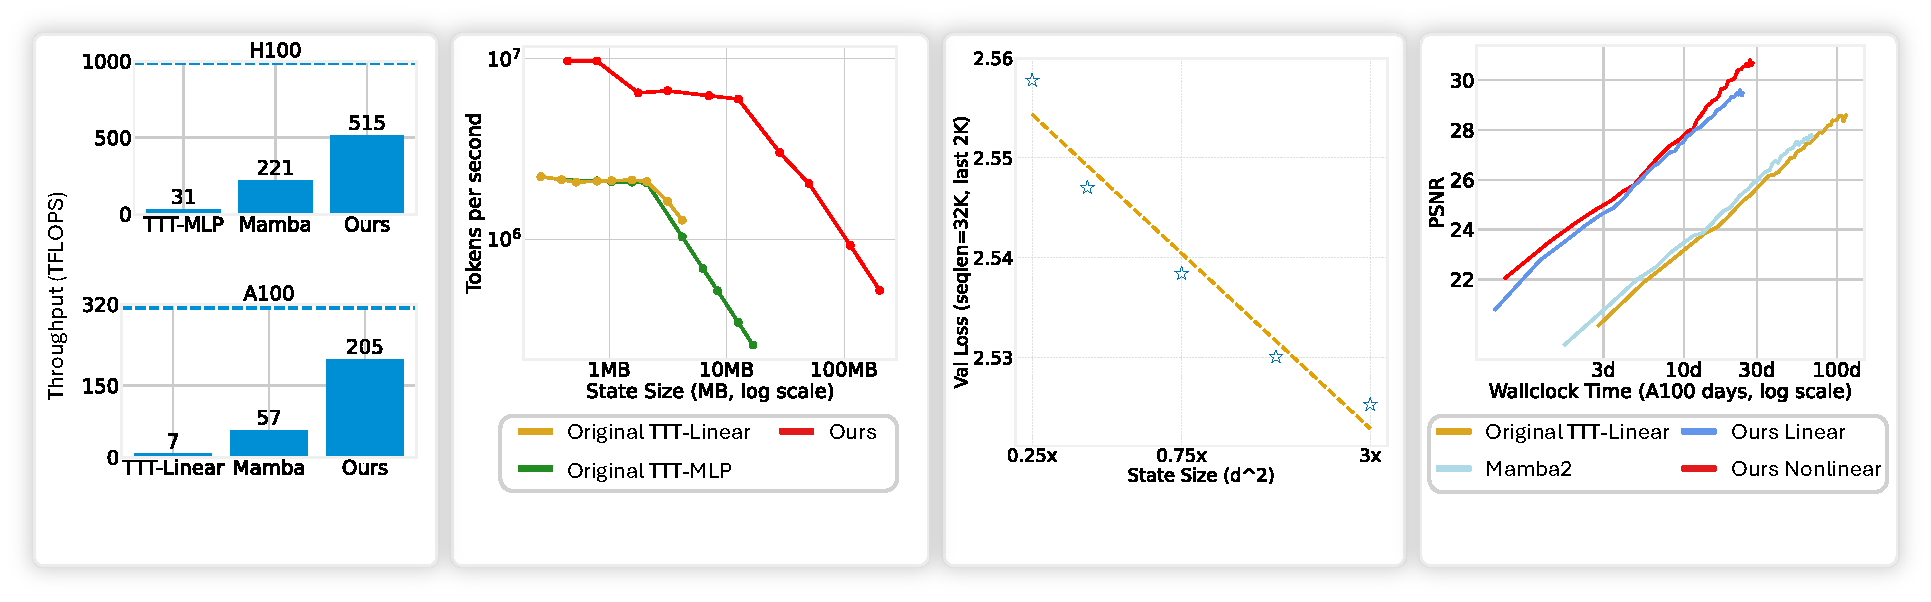
\includegraphics[width=\textwidth]{figures/figure_utilization.pdf}
    \put(-388,12){\capfont \textbf{(a)} GPU Throughput}
    \put(-300,12){\capfont \textbf{(b)} Efficient state scaling}
    \put(-202,12){\capfont \textbf{(c)} Effective state scaling}
    \put(-96,12){\capfont \textbf{(d)} Training Efficiency}
    \vspace{-0.2in}
    \caption{Using larger chunk sizes significantly improves GPU utilization compared to the original test-time training (TTT) method that even uses customized kernels \textbf{(a)}. This enhanced utilization enables efficient and effective scaling to larger state sizes \textbf{(b)}, \textbf{(c)}, leading to better overall performance in less wall-clock time (\textbf{d}). The dotted line in \textbf{(a)} is the theoretical peak BF16 throughput of the GPU. Panel \textbf{(c)} measure average validation loss of the last 2K tokens in sequences processed by a \methodname{} language model across varying state sizes, demonstrating benefits of larger state size. Panel \textbf{(d)} compares performance versus training time across different baselines on the novel view synthesis benchmark. Further experimental details can be found in Sec.~\ref{sec:appen_figure_1_details}.
    \vspace{-0.1in}
    }
    \label{fig:compare_with_ttt}
\end{figure}



On the other hand, a PyTorch-based implementation, while simpler, is typically bounded by memory speed. As an illustration, consider a PyTorch implementation of simple MLP fast weight, the core of which is a matrix multiplication between fast weight (e.g., $h \times h$ matrix) and the mini-batch input ($b \times h$ where b is the chunk size).
The ideal compute-to-memory ratio is:
\begin{align} \label{eq:comp_to_mem_ratio}
r&= \frac{2 h^2 b}{2h^2+ 4 hb}=\frac{h / 2}{1 + \frac{h}{2b}} = \frac{b} {1  + \frac{2b}{h}} \le \min(h / 2, b).
\end{align}
Here, $2 h^2 b$ is the FLOPs to for matrix multiplication, the denominator $2h^2+ 4 hb$ is the memory workload for two input matrices and the output in BF16 (2 bytes).
Small fast weight size (e.g., $h=64$) or small chunk size (e.g., $b=16$) will bound the ratio $r$ far below the theoretical peak (e.g., $290$ FLOPs per byte on H100), making the operation memory-bound and limiting compute usage.

In light of this, we advocate for using large chunk sizes (from $2048$ to $1$M).
This allows us to achieve higher throughput (Fig.~\ref{fig:compare_with_ttt}a) leading to better performance in less training wall-clock time(Fig.~\ref{fig:compare_with_ttt}d).
Our design also allows the state size to be  
scaled up efficiently(Fig.~\ref{fig:compare_with_ttt}b), leading to significant results improvement with such scaling 
(Fig~\ref{fig:compare_with_ttt}c, Fig.~\ref{fig:exp-state-optimizer}a).
Our architecture achieves a state-to-parameter size ratio $\ge\!40\%$, which is an order of magnitude 
larger than previous methods' ratio of $0.1\%$ to $5\%$. Detailed pseudocode is provided in Appendix~\ref{alg:full_lact_layer}.


\textbf{Parallelism over the sequence length dimension}, in addition to the batch and head dimensions, is crucial to achieve high occupancy when handling long sequences (where the batch size is often small). Linear Attention variants like Mamba~\cite{gu2023mamba}, Gated Linear Attention~\cite{yang2024gated} and DeltaNet~\cite{yangparallelizing} enable such parallelism by utilizing the associative property of linear recurrence. Attention~\cite{vaswani2017attention,dao2023flashattention} can be parallelized along the sequence length dimension using online softmax~\cite{milakov2018online}, a key improvement in FlashAttention-2~\cite{dao2023flashattention} over FlashAttention-1~\cite{dao2022flashattention}. For test-time training with non-linear updates, sequence dimension parallelism can only be implemented within online chunks, further motivating the use of extremely large chunk sizes. When implementing large-chunk TTT with PyTorch, this sequence dimension parallelism within a device across multiple thread blocks is automatically handled by PyTorch and low-level compilers. An example of such sequence parallelism across multiple devices is provided in Section~\ref{sec:parallelism}, with pseudocode in Appendix~\ref{alg:lact_chunk_cp}.







